\section{kaneton event manager}

\subsection*{event interface}

\function{}{event\_reserve}{(i\_event \argument{id},
                           e\_event\_type \argument{type},
                           u\_event\_handler \argument{handler})}
	 {
	   Install an event handler.

	   \argument{type} can be :
	   \begin{itemize}
	     \item
	       {\em EVENT\_FUNCTION}:
	       the event calls the function pointed by the union \argument{handler}
	     \item
	       {\em EVENT\_MESSAGE}:
	       the event generates an IPC to the task given in the union \argument{handler}.
	   \end{itemize}

	   The union \argument{handler} contains a pointer to a
	   function returning void and getting an event identifier in
	   argument and an optional error code (integer). The union
	   also contains a task identifier in the case of an IPC action.
	 }

\function{}{event\_release}{(i\_event \argument{id})}
	 {
	   Release an event handler.
	 }

\subsection*{event manager example}

\begin{verbatim}
void          ia32_pf_handler(t_id         id,
                              t_uint32     error_code)
{
  t_uint32    addr;

  SCR2(addr);
  printf("#PF @ %p\n", addr);

  while (1)
    ;
}

...

event_reserve(14, EVENT_FUNCTION, EVENT_HANDLER(ia32_pf_handler));
\end{verbatim}

\newpage

\section{kaneton thread manager}

\subsection*{thread interface}

\function{}{thread\_reserve}{(i\_task \argument{task},
                            t\_prior \argument{prior},
                            i\_thread* \argument{id})}
	 {
	   Reserve a thread for the task \argument{task}
	   given the default thread priority \argument{prior}.

	   Note that once reserved, the thread is marked as stopped.

	   Priority takes its value from \emph{THREAD\_LPRIOR} to \emph{THREAD\_HPRIOR}.
	 }

\function{}{thread\_release}{(i\_thread \argument{id})}
	 {
	   Release the thread object \argument{id}.
	 }

\function{}{thread\_priority}{(i\_thread \argument{id},
                             t\_prior \argument{prior})}
	 {
	   Update the current thread priority to \argument{prior}.

	   Priority takes its value from \emph{THREAD\_LPRIOR} to \emph{THREAD\_HPRIOR}.
	 }

\function{}{thread\_state}{(i\_thread \argument{id},
                          t\_state \argument{sched})}
	 {
	   Stops or start a thread.

	   \argument{sched} values can be:

	   \begin{itemize}
	     \item
	       {\em SCHED\_STATE\_RUN}: run the thread.
	     \item
	       {\em SCHED\_STATE\_STOP}: stop the thread.
	   \end{itemize}
	 }

\function{}{thread\_get}{(i\_thread \argument{id},
                        o\_thread** \argument{o})}
	 {
	   Find the thread object corresponding to \argument{id} and return it in \argument{o}.
	 }

\function{}{thread\_stack}{(i\_thread \argument{id},
                          t\_stack \argument{stack})}
	 {
	   Allocates a stack for the thread \argument{id}.

	   The \argument{stack} argument is a struct containing the
	   size of the stack and a field called \emph{base}. If {\em base}
	   is not equal to 0, then no space is allocated and the stack base
	   is set to the address \argument{base}.
	 }

\function{}{thread\_load}{(i\_thread \argument{id},
                         t\_thread\_context \argument{context})}
	 {
	   Load a new execution context in the thread object \argument{id}.

	   A thread execution context \textit{t\_thread\_context}
	   only contains the \textit{program counter} and the
	   \textit{stack pointer}.
	 }

\newpage

\section{kaneton sched manager}

\subsection*{sched interface}

\function{}{sched\_yield}{(i\_cpu \argument{cpuid})}
	 {
	   Permit the current thread to relinquish the processor voluntarily.

	   Do not care about the argument \argument{cpuid}.
	 }

\function{}{sched\_add}{(i\_thread \argument{thread})}
	 {
	   Adds a runnable thread to the scheduler. Even if the added thread
	   has the highest priority, do not yield the current thread.
	 }

\function{}{sched\_remove}{(i\_thread \argument{thread})}
	 {
	   Remove a thread from the scheduler. \textbf{Be careful:}
	   the thread to remove can be executing.
	 }

\function{}{sched\_update}{(i\_thread \argument{thread})}
	 {
	   Asks the scheduler to update the thread \argument{thread} in its
	   internal data structures since for example the thread's priority
	   just changed.
	 }

\function{}{sched\_current}{(i\_thread* \argument{thread})}
	 {
	   Find the identifier of the currently executing thread and return
	   it in \argument{thread}
	 }

\section{kaneton set manager}

\subsection*{set interface}

\function{}{set\_size}{(i\_set \argument{id},
                      t\_setsz \argument{size})}
	 {
	   Returns in \argument{size} the number of elements in the set.
	 }

\function{}{set\_add}{(i\_set \argument{id},
                     void* \argument{data})}
	 {
	   Adds a data object into the set \argument{id}.
	 }

\function{}{set\_remove}{(i\_set \argument{id},
                        t\_id \argument{i})}
	 {
	   Remove an object identified by \argument{i} from the set
	   \argument{id}.
	 }

\function{}{set\_object}{(i\_set \argument{id},
                        t\_iterator \argument{iterator},
                        void** \argument{data})}
	 {
	   Return the data object matching the iterator.
	 }

\function{}{set\_get}{(i\_set \argument{setid},
                     t\_id \argument{id},
                     void** \argument{o})}
         {
	   Find an element in the set given its identifier \argument{id}.
	 }

\function{}{set\_push}{(i\_set \argument{id},
                      void* \argument{data})}
	 {
	   Add an object to a FIFO or LIFO structure.
	 }

\function{}{set\_pop}{(i\_set \argument{id})}
	 {
	   Remove the next object of a FIFO or a LIFO structure.
	 }

\function{}{set\_pick}{(i\_set \argument{id},
                      void** \argument{data})}
	 {
	   Return the next object of a FIFO or a LIFO structure
	   without deleting it.
	 }

\function{}{set\_reserve}{(\argument{type},
                         t\_opts \argument{opts},
                         t\_size \argument{datasz},
                         i\_set* \argument{id})}
	 {
	   Reserves a set object of type \argument{type}
	   with options \argument{opts} which contains objects of
	   \argument{datasz} size. Its identifier is returned in \argument{id}.

	   \argument{type} values can be:

	   \begin{itemize}
	     \item
	       \emph{ll}: doubly linked-list
	     \item
	       \emph{array}: array
	     \item
	       \emph{pipe}: FIFO
	     \item
	       \emph{stack}: LIFO
	   \end{itemize}
	 }

\function{}{set\_release}{(i\_set \argument{id})}
	 {
	   Release the set \argument{id}.
	 }

\subsection*{set\_foreach example}

\begin{verbatim}
t_state         state;
o_segment       *seg;
t_iterator      i;

set_foreach(SET_OPT_FORWARD, segments, &i, state)
  {
    if (set_object(segments, i, (void**)&seg) != STATUS_OK)
      AS_LEAVE(as, STATUS_UNKNOWN_ERROR);

    // use seg variable here
  }
\end{verbatim}

\newpage

\section{Feuille de r�ponse de l'excercice 3}

Nom :\hspace{5cm}Prenom :\\

\subsection{Round Robin avec priorit� et vieillisement}

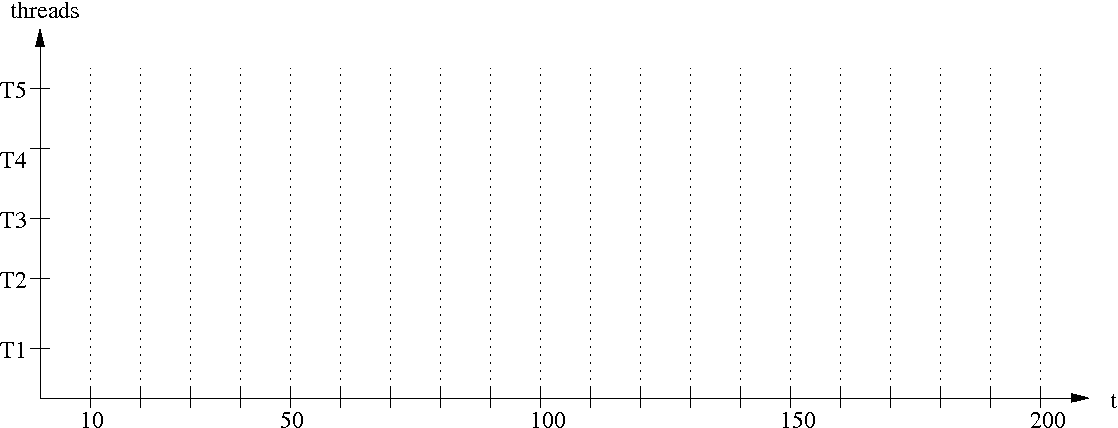
\includegraphics[width=\linewidth]{figures/grid-sched}

\subsection{Multilevel Feedback Queue}

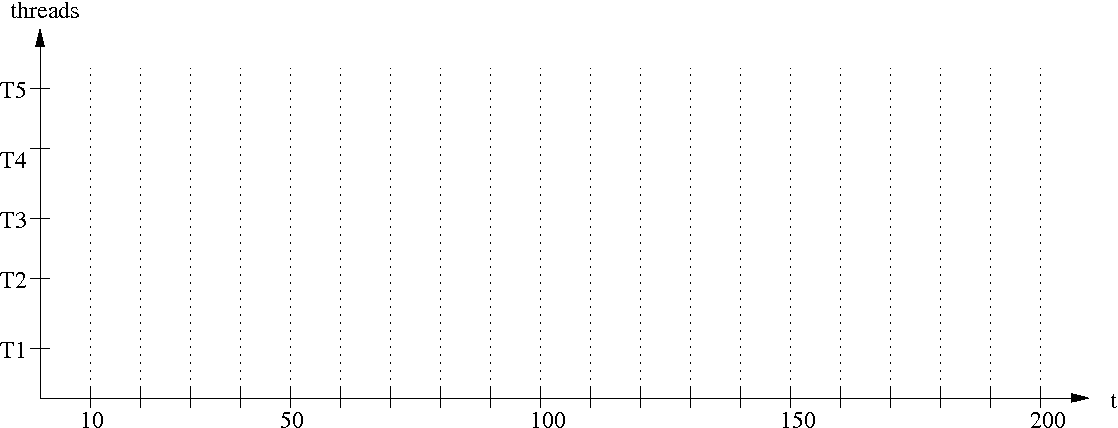
\includegraphics[width=\linewidth]{figures/grid-sched}

\end{document}
